% --------------------------------------------














% --------------------------------------------

\documentclass[a0,portrait]{a0poster}\usepackage[]{graphicx}\usepackage[]{color}
%% maxwidth is the original width if it is less than linewidth
%% otherwise use linewidth (to make sure the graphics do not exceed the margin)
\makeatletter
\def\maxwidth{ %
  \ifdim\Gin@nat@width>\linewidth
    \linewidth
  \else
    \Gin@nat@width
  \fi
}
\makeatother

\definecolor{fgcolor}{rgb}{0.345, 0.345, 0.345}
\newcommand{\hlnum}[1]{\textcolor[rgb]{0.686,0.059,0.569}{#1}}%
\newcommand{\hlstr}[1]{\textcolor[rgb]{0.192,0.494,0.8}{#1}}%
\newcommand{\hlcom}[1]{\textcolor[rgb]{0.678,0.584,0.686}{\textit{#1}}}%
\newcommand{\hlopt}[1]{\textcolor[rgb]{0,0,0}{#1}}%
\newcommand{\hlstd}[1]{\textcolor[rgb]{0.345,0.345,0.345}{#1}}%
\newcommand{\hlkwa}[1]{\textcolor[rgb]{0.161,0.373,0.58}{\textbf{#1}}}%
\newcommand{\hlkwb}[1]{\textcolor[rgb]{0.69,0.353,0.396}{#1}}%
\newcommand{\hlkwc}[1]{\textcolor[rgb]{0.333,0.667,0.333}{#1}}%
\newcommand{\hlkwd}[1]{\textcolor[rgb]{0.737,0.353,0.396}{\textbf{#1}}}%
\let\hlipl\hlkwb

\usepackage{framed}
\makeatletter
\newenvironment{kframe}{%
 \def\at@end@of@kframe{}%
 \ifinner\ifhmode%
  \def\at@end@of@kframe{\end{minipage}}%
  \begin{minipage}{\columnwidth}%
 \fi\fi%
 \def\FrameCommand##1{\hskip\@totalleftmargin \hskip-\fboxsep
 \colorbox{shadecolor}{##1}\hskip-\fboxsep
     % There is no \\@totalrightmargin, so:
     \hskip-\linewidth \hskip-\@totalleftmargin \hskip\columnwidth}%
 \MakeFramed {\advance\hsize-\width
   \@totalleftmargin\z@ \linewidth\hsize
   \@setminipage}}%
 {\par\unskip\endMakeFramed%
 \at@end@of@kframe}
\makeatother

\definecolor{shadecolor}{rgb}{.97, .97, .97}
\definecolor{messagecolor}{rgb}{0, 0, 0}
\definecolor{warningcolor}{rgb}{1, 0, 1}
\definecolor{errorcolor}{rgb}{1, 0, 0}
\newenvironment{knitrout}{}{} % an empty environment to be redefined in TeX

\usepackage{alltt}

\usepackage{marvosym} % Required for symbols in the colored box
\usepackage{ifsym} % Required for symbols in the colored box
\usepackage[usenames,dvipsnames]{xcolor} % Allows the definition of hex colors

% Colors for links, text and headings
\usepackage{hyperref}
\definecolor{linkcolor}{HTML}{0000FF} % Blue-gray color for links
\definecolor{shade}{HTML}{efedf5}
\definecolor{text1}{HTML}{2b2b2b} % Main document font color, off-black
\definecolor{headings}{HTML}{701112} % Dark red color for headings
% Other color palettes: shade=B9D7D9 and linkcolor=A40000; shade=D4D7FE and linkcolor=FF0080

\hypersetup{colorlinks, breaklinks, urlcolor=linkcolor, linkcolor=linkcolor} % Set up links and colors

\usepackage{titlesec} % Allows creating custom \section's

% Format of the section titles
\titleformat{\section}{\color{headings}
\scshape\Large\raggedright}{}{0cm}{}[\color{brown}\titlerule]
\titlespacing{\section}{5pt}{0pt}{5pt} % Spacing around titles

\usepackage{times} % Use the times font
%\usepackage{palatino} % Uncomment to use the Palatino font
\usepackage{graphicx} % Required for including images
\graphicspath{{figure/}} % Location of the graphics files
\usepackage{booktabs} % Top and bottom rules for table
\usepackage[font=small, labelfont=bf]{caption} % Required for specifying captions to tables and figures
\usepackage{amsfonts, amsmath, amsthm, amssymb} % For math fonts, symbols and environments
\usepackage{wrapfig} % Allows wrapping text around tables and figures
\usepackage[flushleft]{threeparttable}
\IfFileExists{upquote.sty}{\usepackage{upquote}}{}
\begin{document}
\color{text1} % Sets the default text color for the whole document to the color defined as 'text1'

%-------------------------------------------------------------------------------------
%	TITLE
%-------------------------------------------------------------------------------------

{\centering \veryHuge \textbf{MortalityLaws R Package} \\ % Title
\Huge\textit{A History of Mortality Modeling from Gompertz to Lee-Carter}\\[1cm]}
{\centering \color{headings} \emph{The 4th Human Mortality Database Symposium, 22 - 23 May 2017, Berlin} \\[30pt]\par} 

\colorbox{shade}{
\begin{tabular}{ l  l }
\Large
\begin{minipage}[t]{0.5\textwidth}
    \textcolor{text1}{
    \begin{tabular}{c|p{33cm}}
    \raisebox{0pt}{\textcircled{a}} & \textbf{Marius Pascariu \& Vladimir Canudas-Romo} \\
    \raisebox{0pt}{\textifsymbol{18}} & \textbf{Max-Planck Odense Center on the Biodemography of Aging} \\
    \raisebox{0pt}{} & \textbf{University of Southern Denmark} \\
    \raisebox{0pt}{\MVAt} & \href{mailto:mpascariu@health.sdu.dk.com}{mpascariu@health.sdu.dk} \\
    \raisebox{0pt}{\Mundus} & \href{https://github.com/mpascariu}{https://github.com/mpascariu} \\ 
    \end{tabular}
    }
\end{minipage}

\begin{minipage}[t]{0.5\textwidth}
\vspace{-100pt}
\centering 
\includegraphics[width = 30cm]{Logos_A.png}\\[1cm]
\end{minipage}

\end{tabular}
}\\


%-------------------------------------------------------------------------------------
\begin{tabular}{ l  l }

\begin{minipage}[t]{0.5\textwidth} % Start the left-hand side of the page
\vspace{0pt} % Trick for alignment
\section*{Mortality modelling timeline}
\begin{knitrout}
\definecolor{shadecolor}{rgb}{0.969, 0.969, 0.969}\color{fgcolor}
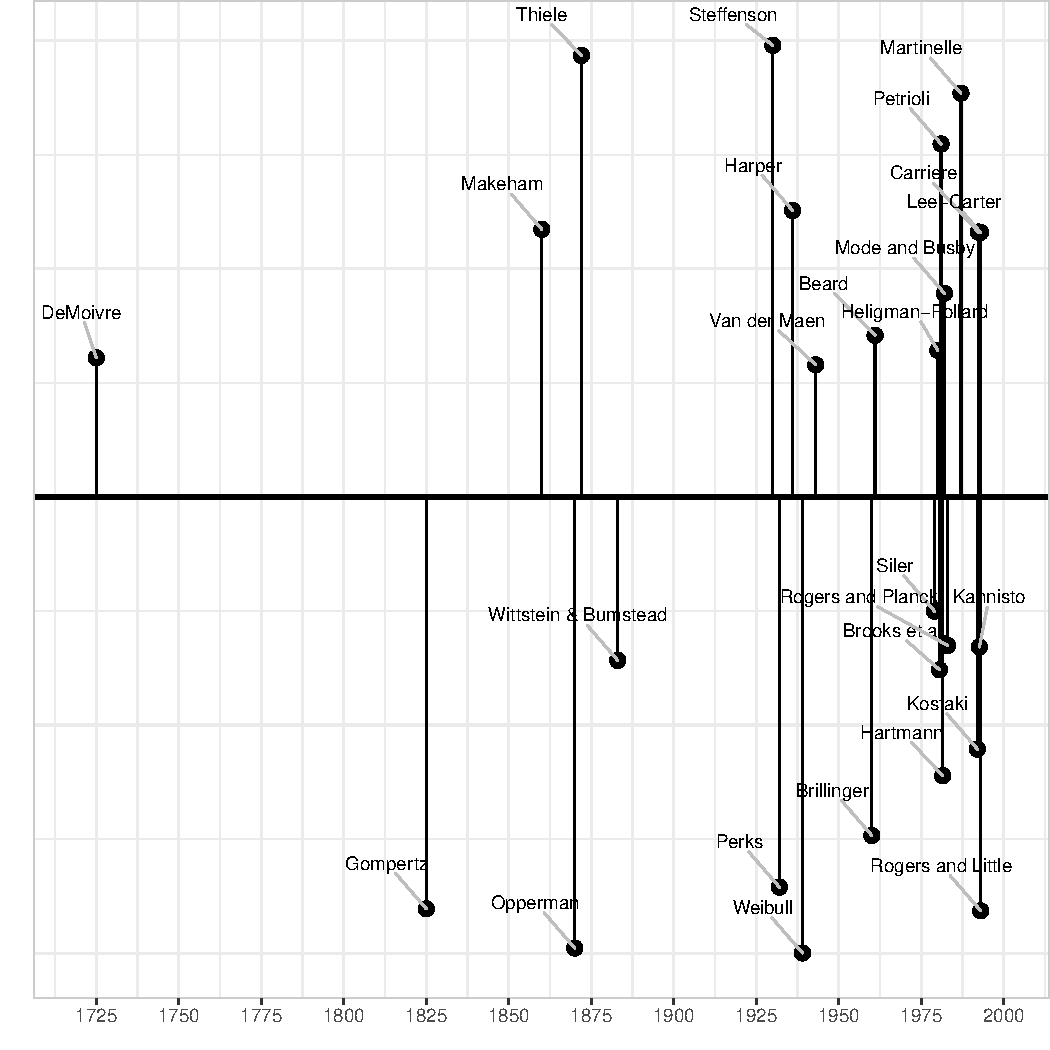
\includegraphics[width=1\linewidth]{figure/plot_timeline-1} 

\end{knitrout}
\end{minipage} % End the left-hand side of the page

% Some space in the midle
\begin{minipage}{0.05\textwidth}
  \begin{tabular}{cc}
  \end{tabular}
\end{minipage}

\begin{minipage}[t]{0.45\textwidth}
  \section*{Main Objective}
  \large
   Build an R package that is capable of performing multiple tasks in a matter of seconds. For example:
  \begin{itemize}
  \item Download and save HMD data;
  \item Fit mortality laws over different age intervals;
  \item Provide multiple fitting procedures for the same model (MLEs, loss functions etc.);
  \item Smooth data;
  \item Construct life tables given different type of input data ($q_x$, $m_x$, $D_x$, $E
  _x$ etc.);
  \item Facilitate comparisons of mortality improvements across time and ages;
  \item Generate instant plots and goodness of fit measures.
  \end{itemize}
  
  
  \section*{The structure of the MoralityLaws R package}
\begin{knitrout}
\definecolor{shadecolor}{rgb}{0.969, 0.969, 0.969}\color{fgcolor}

{\centering 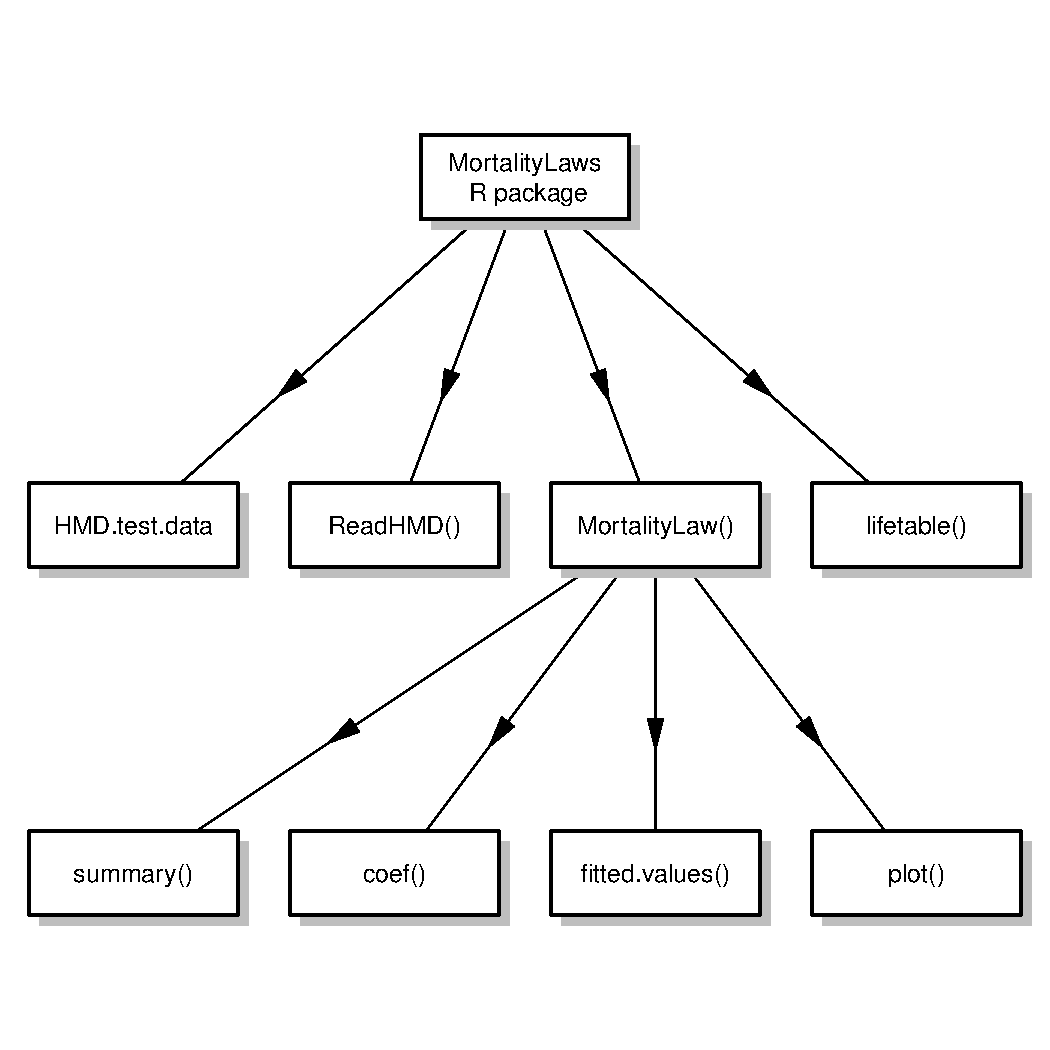
\includegraphics[width=0.75\linewidth]{figure/Diagram-1} 

}



\end{knitrout}
\end{minipage} % End right-hand side of the page

\end{tabular}
%-------------------------------------------------------------------------------------




%------------------------------------------
\begin{wraptable}{r}{0.5\textwidth}
\vspace{-5cm}
\begin{knitrout}
\definecolor{shadecolor}{rgb}{0.969, 0.969, 0.969}\color{fgcolor}
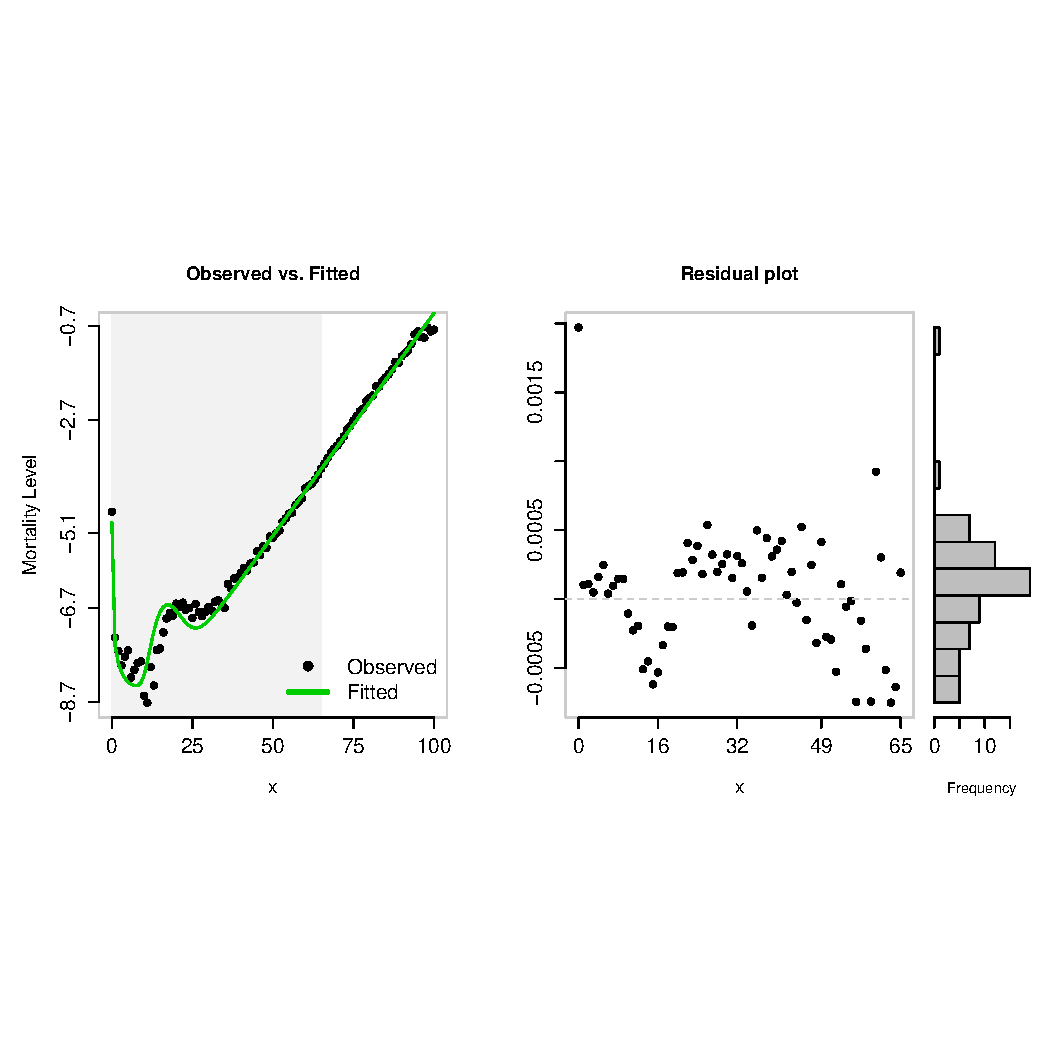
\includegraphics[width=1\linewidth]{figure/unnamed-chunk-3-1} 

\end{knitrout}
\end{wraptable} 



\section*{Implemented Parametric Functions \& Generic Plots}
\begin{table}[h!]
\renewcommand{\arraystretch}{1.4}
\begin{tabular}{lll}
    \toprule \textbf{Mortality laws}  & \textbf{Predictor} & Code\tnote{\textdagger} \\ \hline
    Gompertz & $ae^{bx}$ & \texttt{gompertz0} \\
    Gompertz & $\frac{1}{\sigma }exp\left\{\frac{x-m}{\sigma }\right\}$ & \texttt{gompertz} \\
    Inverse-Gompertz & ${\frac{1}{\sigma }exp\left\{\frac{x-m}{\sigma }\right\}}/{\left(exp\left\{e^{\frac{-(x-m)}{\sigma }}\right\}-1\right)}$ & \texttt{invgompertz}\\
    Makeham & $ae^{bx}+c$ & \texttt{makeham0} \\
    Makeham & $\frac{1}{\sigma }exp\left\{\frac{x-m}{\sigma }\right\} + c$ & \texttt{makeham} \\
    Inverse-Makeham & ${\frac{1}{\sigma }exp\left\{\frac{x-m}{\sigma }\right\}}/{\left(exp\left\{e^{\frac{-(x-m)}{\sigma }}\right\}-1\right)}+c$ & \texttt{invmakeham} \\
    Opperman & $ \frac{a}{\sqrt{x}}+b+c\sqrt[3]{x}$ & \texttt{opperman} \\
    Thiele & $ a_1e^{-b_1x}+\ a_2e^{-\frac{1}{2}b_2{\left(x-c\right)}^2}+a_3e^{b_3x}$ & \texttt{thiele} \\
    Wittstein \& Bumstead & $\frac{1}{m}a^{{-\left(mx\right)}^n}+a^{{-\left(M-x\right)}^n}$ & \texttt{wittstein} \\
    Weibull& $\frac{1}{\sigma }{\left(\frac{x}{m}\right)}^{\frac{m}{\sigma }-1}$ & \texttt{weibull} \\
    Inverse-Weibull & ${\frac{1}{\sigma }{\left(\frac{x}{m}\right)}^{-\frac{m}{\sigma }-1}}/{\left(exp\left\{{\left(\frac{x}{m}\right)}^{-\frac{m}{\sigma }}\right\}-1\right)}$ &  \texttt{invweibull} \\
    Siler  & $a_1e^{-b_1t}+a_2+a_3e^{b_3t}$ & \texttt{siler} \\
    Heligman - Pollard& $\ A^{{\left(x+B\right)}^C}+De^{-E{\left({\mathrm{ln} x\ }-{\mathrm{ln} F\ }\right)}^2}+GH^x$ & \texttt{HP} \\
    Kannisto & $\frac{ae^{bx}}{1+ae^{bx}}+c$ & \texttt{kannisto} \\
    Carriere\tnote{*} & $s\left(x\right)={\psi}_1s_1\left(x\right)+\ {\psi }_2s_2\left(x\right)+\ {\psi }_3s_3\left(x\right)$ & \texttt{carriere1} \\
    \bottomrule
  \end{tabular}

\end{table}



\begin{knitrout}
\definecolor{shadecolor}{rgb}{0.969, 0.969, 0.969}\color{fgcolor}\begin{figure}[!b]

{\centering 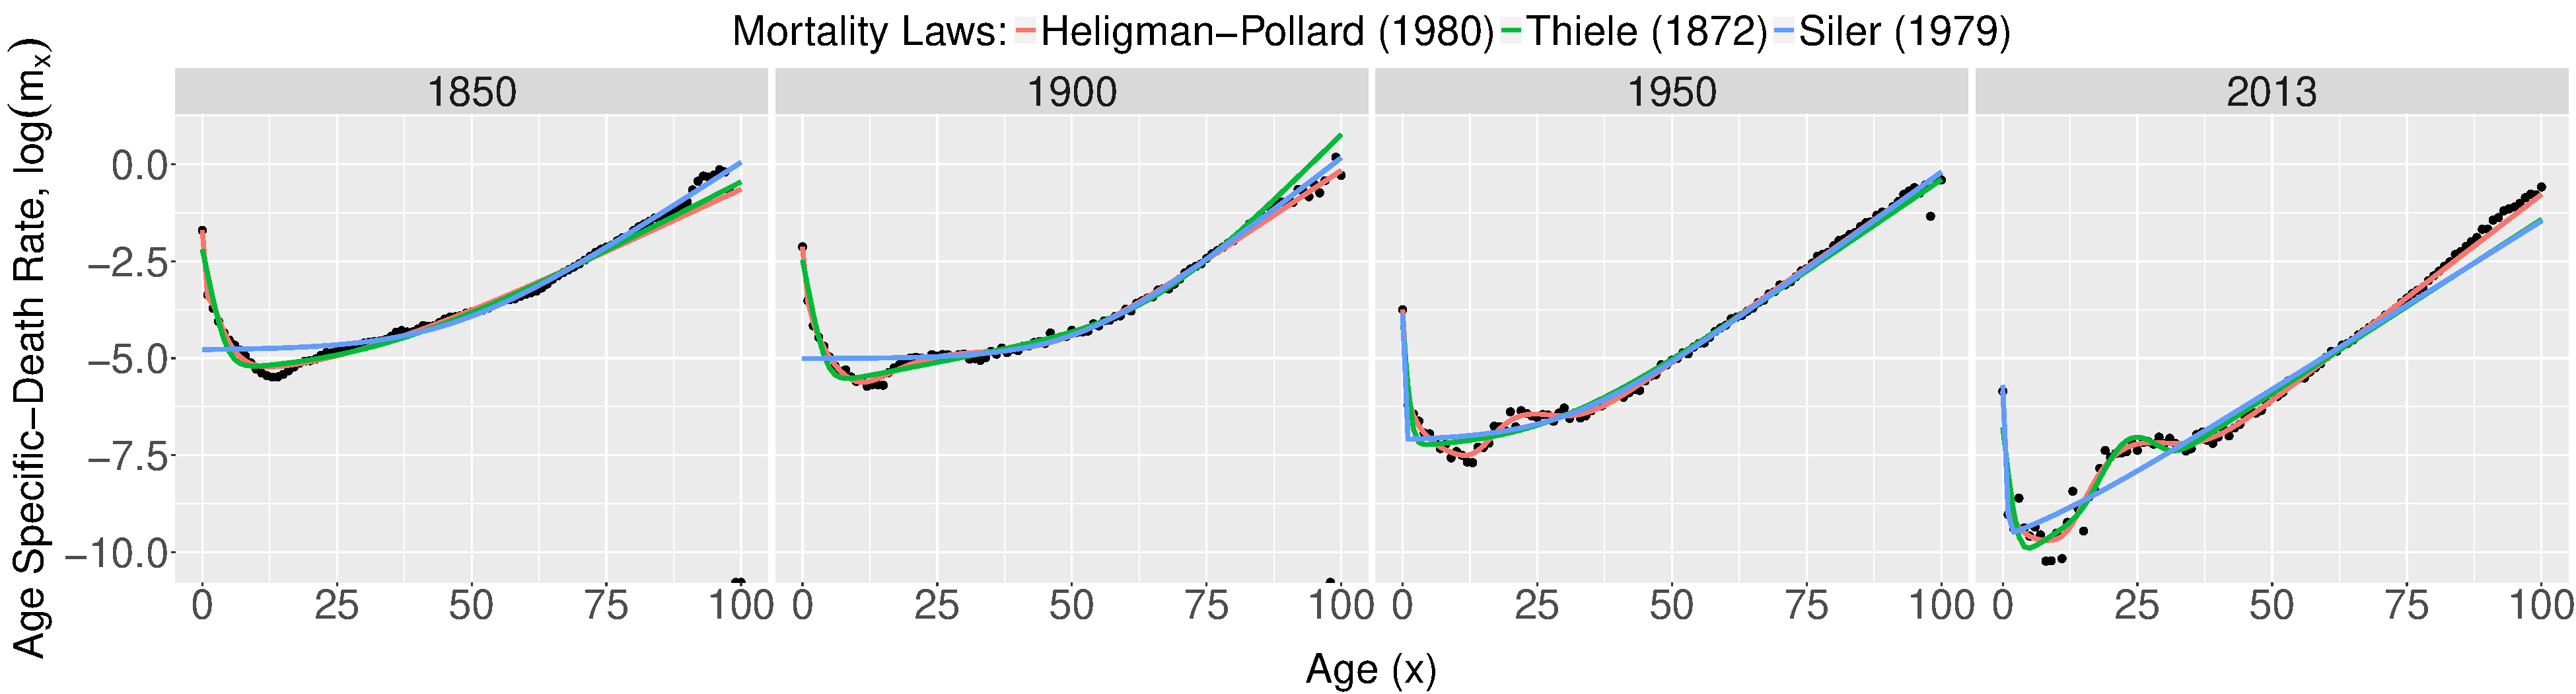
\includegraphics[width=\maxwidth]{figure/gg_full-1} 

}

\caption[Observed and fitted death rates between age 0 and 80 for male population in Sweden]{Observed and fitted death rates between age 0 and 80 for male population in Sweden. The mortality is extrapolated up to age 100.}\label{fig:gg_full}
\end{figure}


\end{knitrout}


\end{document}  
